\documentclass[conference]{IEEEtran}
\IEEEoverridecommandlockouts
% The preceding line is only needed to identify funding in the first footnote. If that is unneeded, please comment it out.
\usepackage{cite}
\usepackage{amsmath,amssymb,amsfonts}
\usepackage{algorithmic}
\usepackage{graphicx}
\usepackage{textcomp}
\usepackage{xcolor}
\usepackage{tabularx}
\def\BibTeX{{\rm B\kern-.05em{\sc i\kern-.025em b}\kern-.08em
T\kern-.1667em\lower.7ex\hbox{E}\kern-.125emX}}
\begin{document}

\title{Optimización en la asignación de vacunas en centros de salud mediante
    una API RESTful basada en el algoritmo de búsqueda de Péndulo\\
}

\author{\IEEEauthorblockN{Carlos Alfredo Castillo Rodriguez}
    \IEEEauthorblockA{\textit{Facultad de Ingeniería, ciencia y tecnología} \\
        \textit{Universidad Bernardo O'higgins}\\
        Santiago, Chile \\
        castilloc@postgrado.ubo.cl}}

\maketitle

\renewcommand{\abstractname}{Resumen}
\begin{abstract}
    \vspace{\baselineskip}

    En los últimos años, existen evidencias de desabastecimiento de
    medicamentos en países subdesarrollados y en vías de desarrollo, por
    razones
    principalmente políticas o climáticas. Dicho desabastecimiento genera
    consecuencias negativas en la salud de la población. En especial en América
    Latina, la falta de vacunas ha sido la principal dificultad para ampliar la
    cobertura de vacunación, debido a la alta dependencia de las importaciones
    de
    medicamentos y materias primas para el desarrollo de tecnologías. Lograr
    minimizar la falta de medicamentos es esencial para garantizar el derecho a
    la
    salud de las personas y fortalecer los programas de prevención y control de
    enfermedades.\par

    Cuando se habla de problemas de optimización, a menudo implican minimizar o
    maximizar recursos tales como pérdidas o ganancias. Estos problemas son
    usualmente complejos y una solución con algoritmos de optimización exactos
    es
    de alto costo computacional.\par

    Este trabajo tiene como objetivo proponer una solución para optimizar la
    distribución de medicamentos en centros de salud utilizando un algoritmo de
    Búsqueda del Péndulo implementado en una API Restful con Node.js y
    MongoDB. La solución propuesta se enfoca en la utilización de la
    metaheurística
    como método de optimización y la implementación de una aplicación web que
    permita a los usuarios realizar la optimización de manera eficiente y
    efectiva.
    Se basó en una revisión bibliográfica exhaustiva de los algoritmos
    metaheurísticos y su aplicación en la optimización de la distribución de
    medicamentos en centros de salud. Se estudió en profundidad el algoritmo de
    Búsqueda del Péndulo y se propuso su implementación en una API Restful
    utilizando Node.js y MongoDB para la optimización de la distribución de
    medicamentos.\par

    La propuesta de solución presentada podría ser una alternativa viable y
    efectiva para resolver el problema de la distribución de medicamentos en
    centros de salud. La utilización de la metaheurística como método de
    optimización permitiría encontrar soluciones óptimas en tiempos razonables
    y
    con costos computacionales acotados. Además, la implementación de una API
    Restful utilizando Node.js y MongoDB permitiría una fácil integración con
    otras
    aplicaciones y sistemas existentes.\par

    En resumen, se propone una solución para optimizar la distribución de
    medicamentos en centros de salud utilizando un algoritmo de Búsqueda del
    Péndulo implementado en una API Restful con Node.js y MongoDB. La solución
    propuesta se enfoca en la utilización de la metaheurística como método de
    optimización y la implementación de una aplicación web eficiente y
    efectiva.
\end{abstract}

\renewcommand{\IEEEkeywords}{Palabras clave}
\begin{IEEEkeywords}
    APIs Restful, Metaheurisitcas, NodeJS, MongoDB, Optimización, Vacunas
\end{IEEEkeywords}

\section{Introducción}

Este trabajo se centra en abordar la creciente crisis de la escasez de
medicamentos esenciales en todo el mundo, la cual ha llevado a malos resultados
sanitarios y al uso inapropiado de medicamentos. El suministro insuficiente en
sistemas de salud, evidente especialmente en América Latina y el Caribe, impide
satisfacer las necesidades de salud pública y de los pacientes. \cite{OMS2016}.

Nuestro objetivo es implementar una solución de software basada en algoritmos
metaheurísticos, particularmente el algoritmo de Búsqueda del Péndulo, para
optimizar la distribución de medicamentos en los centros de salud. La propuesta
es desarrollar una API RESTful utilizando Node.js y MongoDB que implemente este
algoritmo, con el fin de proporcionar una solución que busque la distribución
óptima en tiempos razonables y con costos computacionales acotados.

En el ámbito de la distribución de medicamentos, la optimización juega un papel
fundamental para mejorar la eficiencia y disponibilidad en los centros de
salud. Para abordar este problema, se han utilizado modelos matemáticos y
algoritmos computacionales, entre ellos los algoritmos metaheurísticos, que
proporcionan soluciones aproximadas a problemas complejos de optimización
combinatoria.

En este contexto, este trabajo tiene como objetivo desarrollar una solución de
software basada en metaheurísticas para optimizar la distribución de
medicamentos en centros de salud. Se propone la implementación del algoritmo de
Búsqueda del Péndulo en una API RESTful utilizando Node.js y MongoDB.
Además, se plantea el desarrollo de una aplicación web que utilice esta API
para que los usuarios puedan realizar la optimización de la distribución de
medicamentos de manera eficiente y efectiva, considerando la factibilidad y
viabilidad del modelo propuesto en la situación actual de Chile.

Los objetivos específicos de este trabajo son los siguientes:

\begin{equation}
\text{RMSE} = \sqrt{\frac{1}{n} \sum_{i=1}^{n} (Y_i - \hat{Y}_i)^2}
\end{equation}


\begin{enumerate}
    \item Estudiar a fondo el algoritmo de Búsqueda del Péndulo y entender su
          implementación y parámetros necesarios.
    \item Implementar una API RESTful que incluya la implementación del
          algoritmo para la optimización de la distribución de medicamentos en
          centros de
          salud.
    \item Realizar pruebas y evaluaciones del algoritmo en la API en diferentes
          escenarios de distribución de medicamentos para validar su eficacia y
          eficiencia.
    \item Generar una interfaz visual con Swagger para facilitar el uso de la
          API por parte de los usuarios.
    \item Evaluar la factibilidad y viabilidad de la aplicación web
          desarrollada, teniendo en cuenta aspectos como la escalabilidad,
          seguridad,
          usabilidad y costos.
\end{enumerate}

\section{Marco teórico}
\label{sec:MT}

\subsection{Metaheurística}
En términos generales, una metaheurística es una técnica de optimización que se
utiliza para resolver problemas combinatorios complejos en los que el número de
posibles soluciones es muy grande. Las metaheurísticas son algoritmos de
propósito general que se basan en principios heurísticos y estrategias de
búsqueda no deterministas para encontrar soluciones óptimas o subóptimas en un
tiempo razonable.

A diferencia de los algoritmos de búsqueda exacta, que garantizan la obtención
de la solución óptima en un tiempo finito, pero pueden ser demasiado costosos
computacionalmente para problemas grandes, las metaheurísticas no garantizan la
solución óptima, pero son capaces de encontrar soluciones aceptables en tiempos
mucho más cortos.

Una metaheurística es un marco algorítmico de alto nivel e independiente del
problema que proporciona un conjunto de directrices o estrategias para
desarrollar algoritmos de optimización heurísticos. Son una alternativa viable,
y a menudo superior, a los métodos más tradicionales de optimización
mixta-entera, como la ramificación y acotación y la programación dinámica.
Especialmente para problemas complicados o instancias de problemas grandes, las
metaheurísticas suelen ofrecer una mejor relación entre la calidad de la
solución y el tiempo de cómputo. Además, las metaheurísticas son más flexibles
que los métodos exactos en dos aspectos importantes. En primer lugar, debido a
que los marcos metaheurísticos están definidos en términos generales, los
algoritmos metaheurísticos pueden adaptarse a las necesidades de la mayoría de
los problemas de optimización de la vida real en términos de calidad de
solución esperada y tiempo de cómputo permitido, que pueden variar ampliamente
entre diferentes problemas y situaciones diferentes. En segundo lugar, las
metaheurísticas no imponen ninguna exigencia sobre la formulación del problema
de optimización (como requerir que las restricciones o las funciones objetivo
se expresen como funciones lineales de las variables de decisión). Sin embargo,
esta flexibilidad requiere una considerable adaptación específica del problema
para lograr un buen rendimiento\cite{soerensen2010}.

Un peso de inercia decreciente con el tiempo es un ejemplo de un mecanismo
adoptado con frecuencia por los investigadores para controlar el comportamiento
de los agentes y favorecer la exploración al inicio de la búsqueda antes de
cambiar a la explotación \cite{eberhart2000, bansal2011,
    elkhateeb2013}. El peso de inercia decreciente con el tiempo reduce el
tamaño del paso a medida que aumenta la
iteración. Entre los patrones comunes aplicados por los investigadores se
encuentran el peso de inercia decreciente linealmente y el peso de inercia
decreciente exponencialmente\cite{bansal2011}.

\subsection{Node.js}
Node.js es un entorno de ejecución de código abierto que permite la
programación del lado del servidor utilizando JavaScript. Proporciona un modelo
de programación basado en eventos y un sistema de gestión de paquetes
integrado, facilitando el desarrollo de aplicaciones escalables y de alta
concurrencia \cite{shah2017}.

\subsection{MongoDB}
MongoDB es un sistema de gestión de bases de datos NoSQL orientado a documentos
que proporciona un alto rendimiento de lectura y escritura. Utiliza un formato
similar a JSON llamado BSON, que se adapta naturalmente a las metodologías de
programación orientadas a objetos. Soporta consultas complejas y ofrece
características como fragmentación automática y replicación
\cite{krishnan2016}.

\subsection{JSON Web Tokens (JWT)}
Los JSON Web Tokens son un mecanismo de autenticación y autorización que
codifica un conjunto de afirmaciones como un objeto JSON en una estructura. Se
utilizan en aplicaciones web para mantener a los usuarios autenticados y
autorizados durante su sesión \cite{IETF2015}.

\subsection{RESTful API}
Las APIs RESTful son interfaces de programación basadas en HTTP que permiten la
creación, lectura, actualización y eliminación de recursos. Se utilizan en el
diseño de microservicios y admiten la interoperabilidad y la WWW. Los
principios de REST, como la interfaz uniforme y la identificación de recursos,
permiten una arquitectura simple y escalable \cite{ehsan2022}.

\subsection{Algoritmo de búsqueda del péndulo}
El movimiento armónico del péndulo que oscila centrado en un punto pivote se
imita en este algoritmo. Donde la amplitud del movimiento armónico en ambos
lados del pivote es igual, va amortiguándose y disminuyéndose con el tiempo.
Este comportamiento es imitado por los agentes del algoritmo de búsqueda del
péndulo para moverse y buscar una solución de optimización dentro de un área de
búsqueda. La alta amplitud al principio fomenta la exploración y amplía el área
de búsqueda, mientras que mientras que la baja amplitud hacia el final fomenta
el ajuste fino y la explotación. \cite{aziz2022}.
El movimiento armónico del péndulo amortiguado es la inspiración del algoritmo.
El peso oscila de un lado a otro, mientras que la amplitud de la oscilación
disminuye con el tiempo hasta que se alcanza el equilibrio. La resistencia del
aire amortigua y desacelera el movimiento del péndulo. \cite{aziz2022}.

La imagen 1 ilustra un péndulo oscilante colgado de una cuerda y su típica
oscilación armónica.
\begin{figure}[h!]
    \centering
    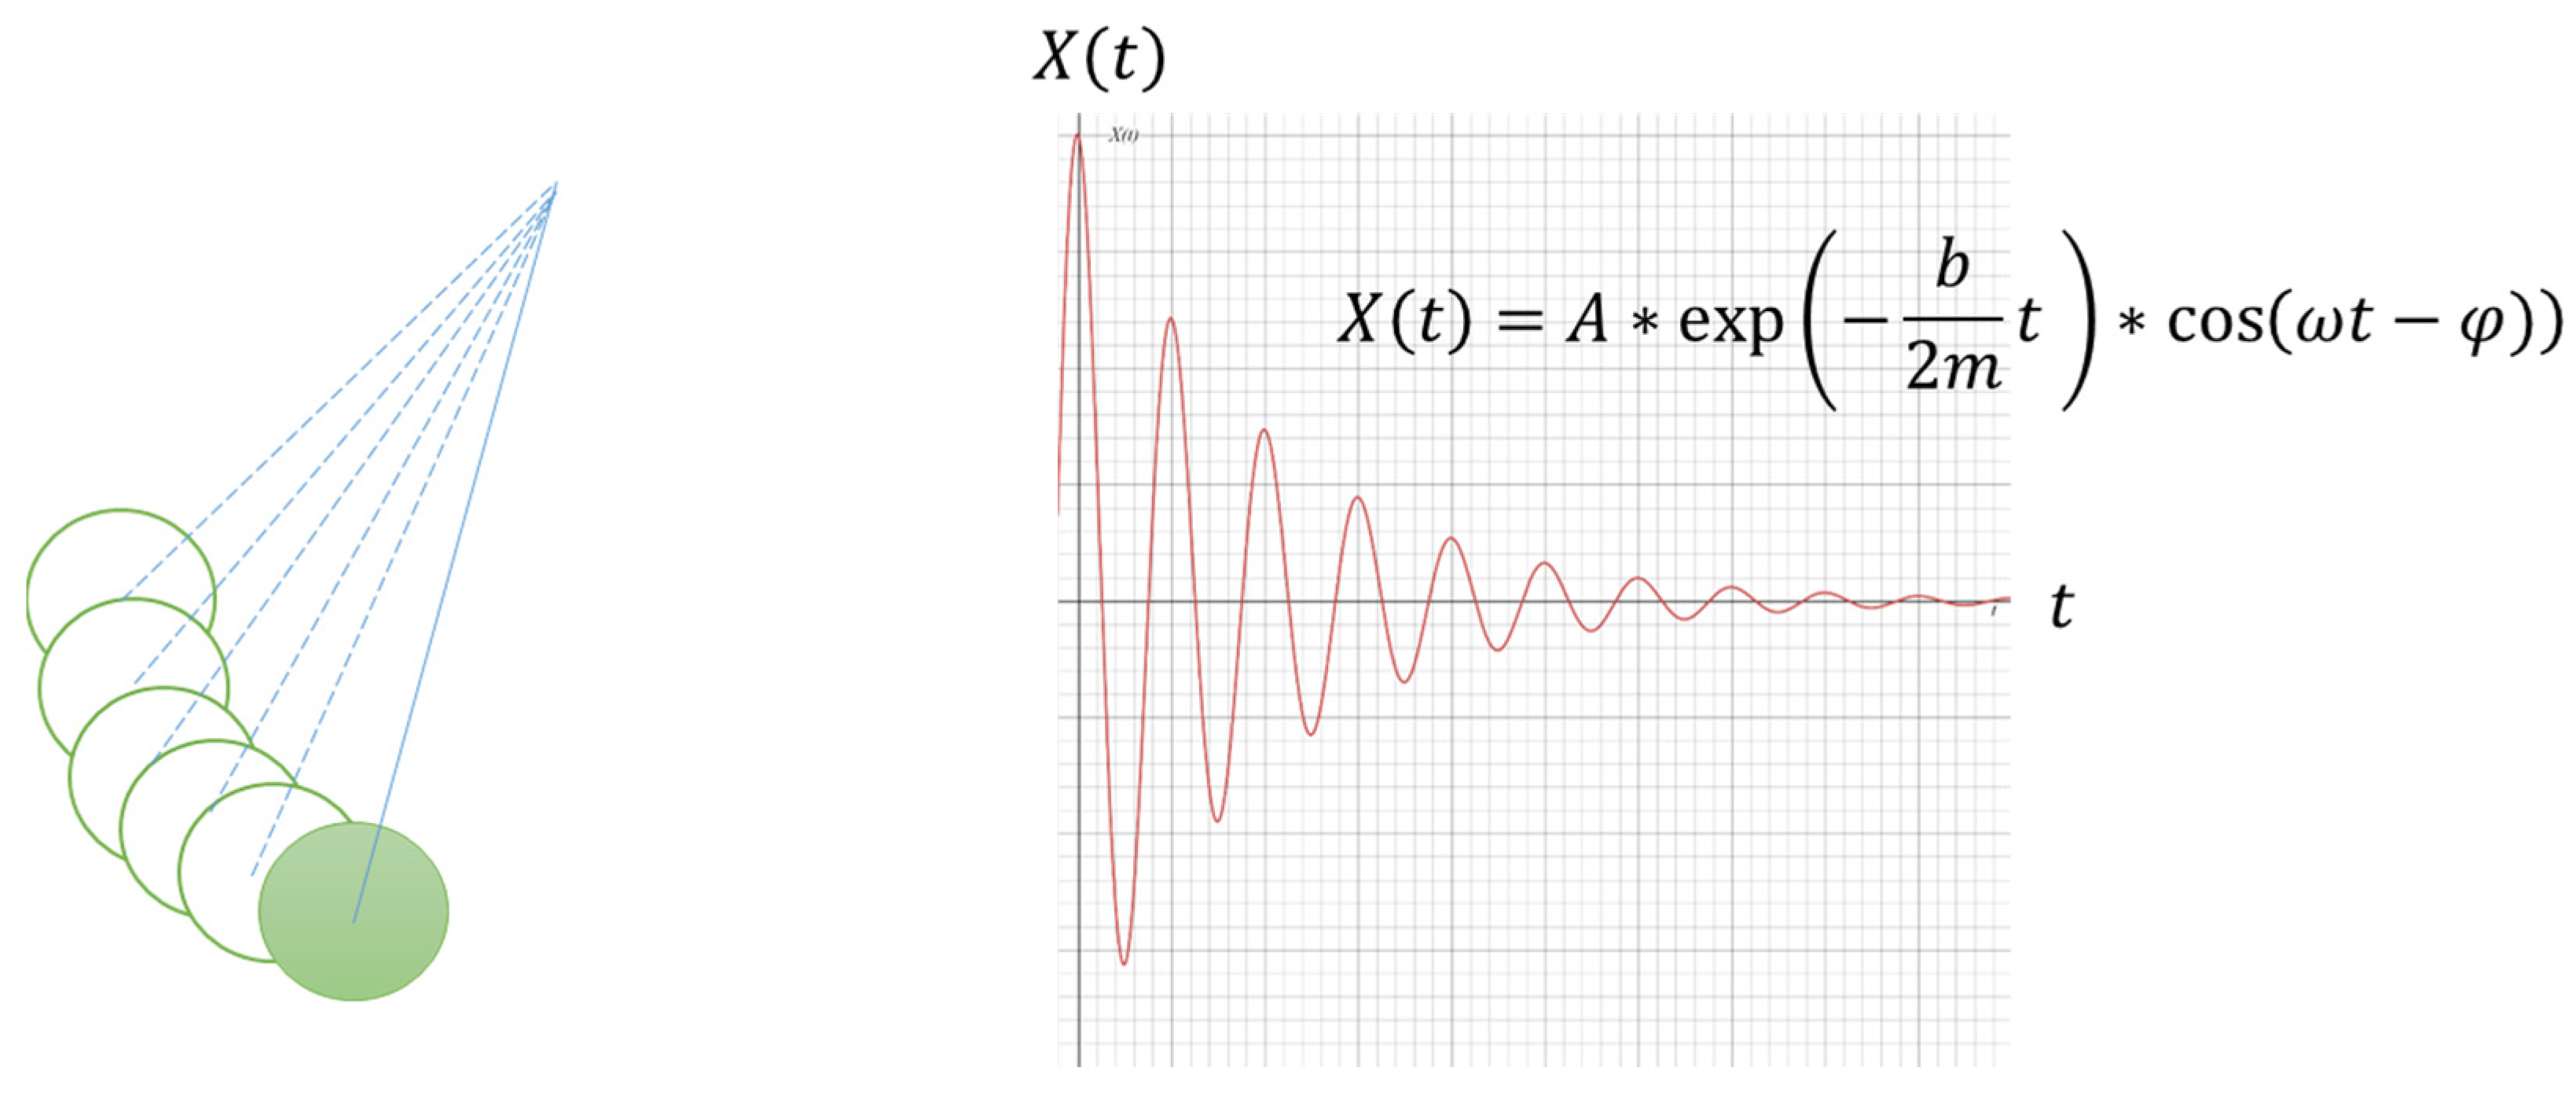
\includegraphics[width=0.5\textwidth, keepaspectratio]{Figures/image1.png}
    \caption{Movimiento armonico del péndulo. \cite{aziz2022}}
    \label{fig:mi_etiqueta}
\end{figure}

Según \cite{aziz2022} La ecuación de la oscilación armónica se muestra en la
formula 1, es una ecuación de movimiento armónico simple amortiguado, donde:

\begin{enumerate}
    \item $X(t)$ es la posición del objeto en función del tiempo.
    \item $A$ es la amplitud de la oscilación, que representa la distancia
          máxima que el objeto se desplaza desde su posición de equilibrio.
    \item $b$ es el coeficiente de amortiguamiento, que determina la rapidez
          con que se desvanece la amplitud de la oscilación debido al
          rozamiento del
          objeto con el medio en el que se encuentra.
    \item $m$ es la masa del objeto en movimiento.
    \item $t$ es el tiempo transcurrido desde el inicio del movimiento.
    \item $\omega$ es la frecuencia angular, que determina la velocidad a la
          que se mueve el objeto en función del tiempo.
    \item $\phi$ es la fase inicial de la oscilación, que representa el desfase
          entre el movimiento y su punto de partida.
\end{enumerate}

La ecuación es:

\begin{equation}
    X(t) = A \cdot e^{-\frac{b}{2m} \cdot t} \cdot \cos(\omega t - \phi)
\end{equation}

El movimiento armónico del péndulo es elegido aquí para controlar el paso de
búsqueda de los agentes del algoritmo debido al patrón oscilante observado.
Este patrón que se expande y se contrae alternadamente mientras disminuye la
amplitud a lo largo del tiempo es deseable. Se predice que este comportamiento
apoyará la exploración de los agentes al principio, y será equilibrado por la
explotación a medida que avance la búsqueda
El algoritmo presentado es una metaheurística basada en población, donde la
búsqueda de la solución óptima es manejada por un grupo de agentes. Cada uno de
los agentes, actúa como un péndulo, con parámetros independientes. Ellos se
mueven alrededor del espacio de búsqueda, buscando el punto de solución optimo,
impulsado por el movimiento del péndulo, que se centra alrededor de su propia
posición actual.

La posición del agente es calculada por medio de la siguiente
ecuación\cite{aziz2022}:

\begin{equation}
    P_i^d (t) = P_i^d (t-1) + \text{pend}_i^d (t) \cdot (\text{Best}^d - P_i^d
    (t-1))
\end{equation}

Donde $P_i^d (t)$ representa la posición del agente $i$ en la dimensión $d$ en
el tiempo $t$ mientras que $\text{Best}^d$ representa la mejor solución
encontrada desde el inicio de la búsqueda en toda la población. El agente se
acerca o se aleja de la mejor solución en función de $\text{pend}_i^d$. Este
último es un valor numérico aleatorio, con la amplitud máxima que oscila
obedeciendo la ecuación armónica del péndulo. Todos los agentes tienen un
$\text{pend}_i^d$ diferente y es calculado por medio de la siguiente ecuación.
\cite{aziz2022}:

\begin{equation}
    \text{pend}_i^d (t) = 2 \exp\left(-\frac{t}{t_{\text{max}}}\cos(2\pi \cdot
    \text{rand})\right)
\end{equation}

\begin{figure}[h!]
    \centering
    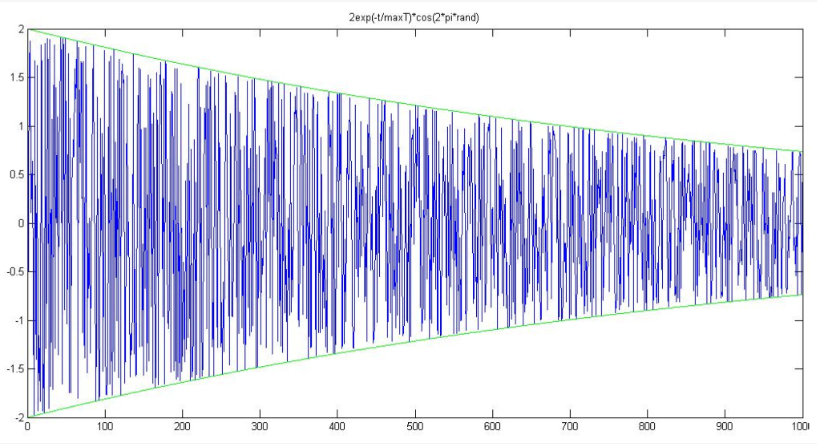
\includegraphics[width=0.5\textwidth, keepaspectratio]{Figures/image2.png}
    \caption{Magnitud de oscilaciones de $\text{pend}_i^d (t)$.
        \cite{aziz2022}}
    \label{fig:mi_etiqueta}
\end{figure}

Esta ecuación imita la ecuación armónica, $t_{\text{max}}$ es el número máximo
de
iteraciones, y \texttt{rand} es un número aleatorio proveniente de una
distribución uniforme. La amplitud máxima de desplazamiento 2 se elige de tal
manera que la exploración sea favorecida durante las primeras iteraciones. Una
vez que $\text{pend}_i^d (t)$ está por debajo de 1, los agentes cambian a
favorecer la explotación. Además, $\text{pend}_i^d (t)$ oscila entre el rango
positivo y negativo. Un valor positivo de $\text{pend}_i^d (t)$ anima a un
agente a moverse hacia la dirección de la mejor solución, mientras que un
$\text{pend}_i^d (t)$ negativo impulsa a los agentes en la dirección opuesta de
la mejor solución \cite{aziz2022}.

Solo se emplean dos ecuaciones matemáticas simples en el algoritmo de búsqueda
del péndulo con dos parámetros a seleccionar, el número de agentes y el número
máximo de iteraciones. Esto hace que sea un algoritmo de optimización muy
simple con bajo costo computacional \cite{aziz2022}.

El pseudocódigo del algoritmo es mostrado en la siguiente tabla:

\renewcommand{\tablename}{Tabla}
\begin{table}[h]
    \centering
    \begin{tabular}{|c|l|}
        \hline
        \textbf{Paso} & \textbf{Acción}
        \\
        \hline
        1             & Inicializar aleatoriamente los parámetros y las
        posiciones de los agentes.                                           \\
        2             & Para i = 1 hasta el número máximo de iteraciones:
        \\
        3             & \hspace{1em} Para cada agente:
        \\
        4             & \hspace{2em} Actualizar el agente usando la ecuación
        (1) y (2).                                                           \\
        5             & \hspace{2em} Evaluar el valor de aptitud del agente.
        \\
        6             & \hspace{1em} Fin del ciclo para cada agente.
        \\
        7             & \hspace{1em} Identificar el mejor agente.
        \\
        8             & Fin del ciclo para i.
        \\
        9             & Solución: mejor agente.
        \\
        \hline
    \end{tabular}
    \caption{Pseudocódigo del Algoritmo de Búsqueda del Péndulo.}
    \label{table:pendulumSearchAlgorithm}
\end{table}

\section{Resultados}
\label{sec:Res}

\subsection{Optimización de Problemas Benchmark}

Según \cite{aziz2022} El rendimiento del algoritmo de Búsqueda del Péndulo
propuesto se estudia utilizando 13
funciones
multimodales del conjunto de pruebas de referencia CEC2014, funciones 4--16.
Estas funciones son problemas de minimización que se desplazan y rotan desde
sus funciones básicas originales. El desplazamiento y la rotación evitan el
problema del sesgo de origen. Las funciones multimodales tienen muchos óptimos
locales y un óptimo global final. Las funciones multimodales son adecuadas para
observar si un algoritmo es capaz de realizar y evitar la convergencia
prematura o no, así como para observar la capacidad de exploración y
explotación del algoritmo. Por lo tanto, solo se adoptan aquí las 14 funciones
multimodales. Los nombres y la idoneidad ideal de las funciones se enumeran en
la Tabla 1; otros detalles de las 13 funciones de referencia, como sus
funciones matemáticas, se pueden encontrar en \cite{Liang2013}.

\renewcommand{\tablename}{Tabla}
\begin{table}[h]
    \centering
    \begin{tabularx}{0.5\textwidth}{|X|c|}
        \hline
        \textbf{Nombre de la Función}
         & \textbf{Aptitud Ideal} \\
        \hline
        f4: Shifted and Rotated Rosenbrock’s Function
         & 400                    \\
        f5: Shifted and Rotated Ackley’s Function
         & 500                    \\
        f6: Shifted and Rotated Weierstrass Function
         & 600                    \\
        f7: Shifted and Rotated Griewank’s Function
         & 700                    \\
        f8: Shifted Rastrigin’s Function
         & 800                    \\
        f9: Shifted and Rotated Rastrigin’s Function
         & 900                    \\
        f10: Shifted Schwefel’s Function
         & 1000                   \\
        f11: Shifted and Rotated Schwefel’s Function
         & 1100                   \\
        f12: Shifted and Rotated Katsuura Function
         & 1200                   \\
        f13: Shifted and Rotated HappyCat Function
         & 1300                   \\
        f14: Shifted and Rotated HGBat Function
         & 1400                   \\
        f15: Shifted and Rotated Expanded Griewank’s plus Rosenbrock’s Function
         & 1500                   \\
        f16: Shifted and Rotated Expanded Scaffer’s F6 Function
         & 1600                   \\
        \hline
    \end{tabularx}
    \caption{Nombres de las funciones y su aptitud ideal.}
    \label{table:functions}
\end{table}

\subsection{Número de Agentes}
Según \cite{aziz2022} Solo hay dos parámetros que seleccionar para el algoritmo
de busqueda del péndulo. El
primero es el número de iteraciones. Este está relacionado con la capacidad
computacional de la plataforma de cálculo y la complejidad de los problemas.
Por tanto, para este experimento, el número de iteraciones se establece en
1000. El segundo parámetro es el número de agentes. En esta sección se
investiga el efecto del número de agentes. Los números de agentes probados son
10, 20, 30, 40 y 50. Todos los ajustes se ejecutan 30 veces; los mejores
resultados de la ejecución se tabulan en la Tabla 3. Dado que las funciones de
referencia son problemas de minimización, los mejores resultados son el valor
mínimo de las 30 ejecuciones de cada configuración. Se puede observar que no
hay un número de agentes que funcione mejor para todas las funciones de prueba.
Sin embargo, el número de agentes igual a 50 obtuvo un mayor número de mejores
resultados en comparación con los demás.

\renewcommand{\tablename}{Tabla}
\begin{table}[h]
    \centering
    \resizebox{0.5\textwidth}{!}{%
        \begin{tabular}{lccccc}
            \hline
            \textbf{Nombre de la Función} & \multicolumn{5}{c}{\textbf{Número
                    de Agentes}}
            \\
                                          & \textbf{10}
                                          & \textbf{20}                       &
            \textbf{30}                   & \textbf{40}                       &
            \textbf{50}                                                         \\
            \hline
            f4                            & 400.0557
                                          & 400.0003                          &
            400.001                       & 400.0008                          &
            400.0013                                                            \\
            f5                            & 519.997
                                          & 519.996                           &
            519.9923                      & 519.983                           &
            519.9913                                                            \\
            f6                            & 601.5922
                                          & 601.0678                          &
            600.3217                      & 600.3587                          &
            600.0771                                                            \\
            f7                            & 700.0595
                                          & 700.027                           &
            700.0418                      & 700.0591                          &
            700.0517                                                            \\
            f8                            & 801.9904
                                          & 800                               &
            800                           & 800                               &
            800                                                                 \\
            f9                            & 905.9708
                                          & 905.9698                          &
            904.9748                      & 905.9698                          &
            904.9748                                                            \\
            f10                           & 1007.031
                                          & 1000.375                          &
            1000.25                       & 1003.602                          &
            1000.25                                                             \\
            f11                           & 1247.431
                                          & 1226.78                           &
            1140.238                      & 1222.493                          &
            1131.949                                                            \\
            f12                           & 1200.059
                                          & 1200.006                          &
            1200.012                      & 1200.01                           &
            1200.017                                                            \\
            f13                           & 1300.138
                                          & 1300.132                          &
            1300.1                        & 1300.043                          &
            1300.137                                                            \\
            f14                           & 1400.171
                                          & 1400.144                          &
            1400.123                      & 1400.079                          &
            1400.052                                                            \\
            f15                           & 1500.94
                                          & 1500.575                          &
            1500.499                      & 1500.578                          &
            1500.417                                                            \\
            f16                           & 1602.263
                                          & 1602.072                          &
            1602.032                      & 1601.511                          &
            1601.108                                                            \\
            \hline
            \textbf{Friedman Rank}        & 5
                                          & 2.9615                            &
            2.3462                        & 2.5769                            &
            2.1154                                                              \\
            \hline
        \end{tabular}%
    }
    \caption{Resultados de las funciones con diferentes números de agentes}
    \label{tab:agentes}
\end{table}

El test de rango con signo de Friedman de 1 × N se realiza entonces para
identificar el mejor número de agentes utilizando este conjunto de funciones de
referencia. El test de rango con signo de Friedman es un método estadístico
comúnmente utilizado para proporcionar un análisis imparcial del rendimiento de
las metaheurísticas \cite{alcala-fdez2009, triguero2017, alcala-fdez2011}.
Cuanto menor sea el rango de Friedman de un algoritmo, mejor será el algoritmo.
Un test de 1 × N compara el algoritmo mejor clasificado con los demás
algoritmos. Si el valor estadístico de Friedman, que se distribuye de acuerdo a
$\chi^2$ con $k-1$ grados de libertad, donde $k$ es el número de prueba (aquí
$k=5$, es decir, 5 número de agentes probados), tiene un valor p menor que el
nivel de significancia adoptado, $\alpha$, entonces se rechaza la hipótesis
nula que afirma que todos los ajustes probados están a la par entre sí. Para
identificar la diferencia significativa, se adopta un procedimiento post-hoc
conocido como procedimiento post-hoc de Holm. En este trabajo, se adopta
$\alpha=0.05$. Además de 0.05, 0.1 también es comúnmente usado por los
investigadores. Cuanto menor sea el valor, más estricto será el test
estadístico en la aceptación de la hipótesis nula.

Según \cite{aziz2022} para el algoritmo debusqueda del pendulo, se realizo el
test estadístico
utilizando Knowledge Extraction based on Evolutionary Learning (KEEL), que es
una herramienta de código abierto
con módulos de análisis estadístico \cite{alcala-fdez2009, triguero2017,
    alcala-fdez2011}. KEEL es un software amigable para el usuario desarrollado
por
un grupo de investigadores para fines de investigación y académicos
\cite{alcala-fdez2009, triguero2017, alcala-fdez2011}.

Los rangos de Friedman se muestran en la última fila de la Tabla 3. El valor
estadístico de Friedman (distribuido de acuerdo con $\chi^2$ con 4 grados de
libertad) es 28.030769 y su valor p es 0.000012, que es menor que un nivel de
significancia de 0.05. Por lo tanto, existe una diferencia significativa entre
los cinco ajustes. El post-hoc de Holm se utiliza para determinar qué ajuste es
igual o peor que el número de agentes mejor clasificado. La Tabla 3 muestra el
valor p y el valor de Holm del test post-hoc. El procedimiento de Holm rechaza
aquellas hipótesis que tienen un valor p < Holm. Por lo tanto, un número de
agentes igual a 10 es significativamente peor que 50, y los demás están a la
par entre sí. Por lo tanto, se puede concluir que se recomienda un número de
agentes superior a 20 para el algoritmo de busqueda del péndulo.

\begin{figure}[h!]
    \centering
    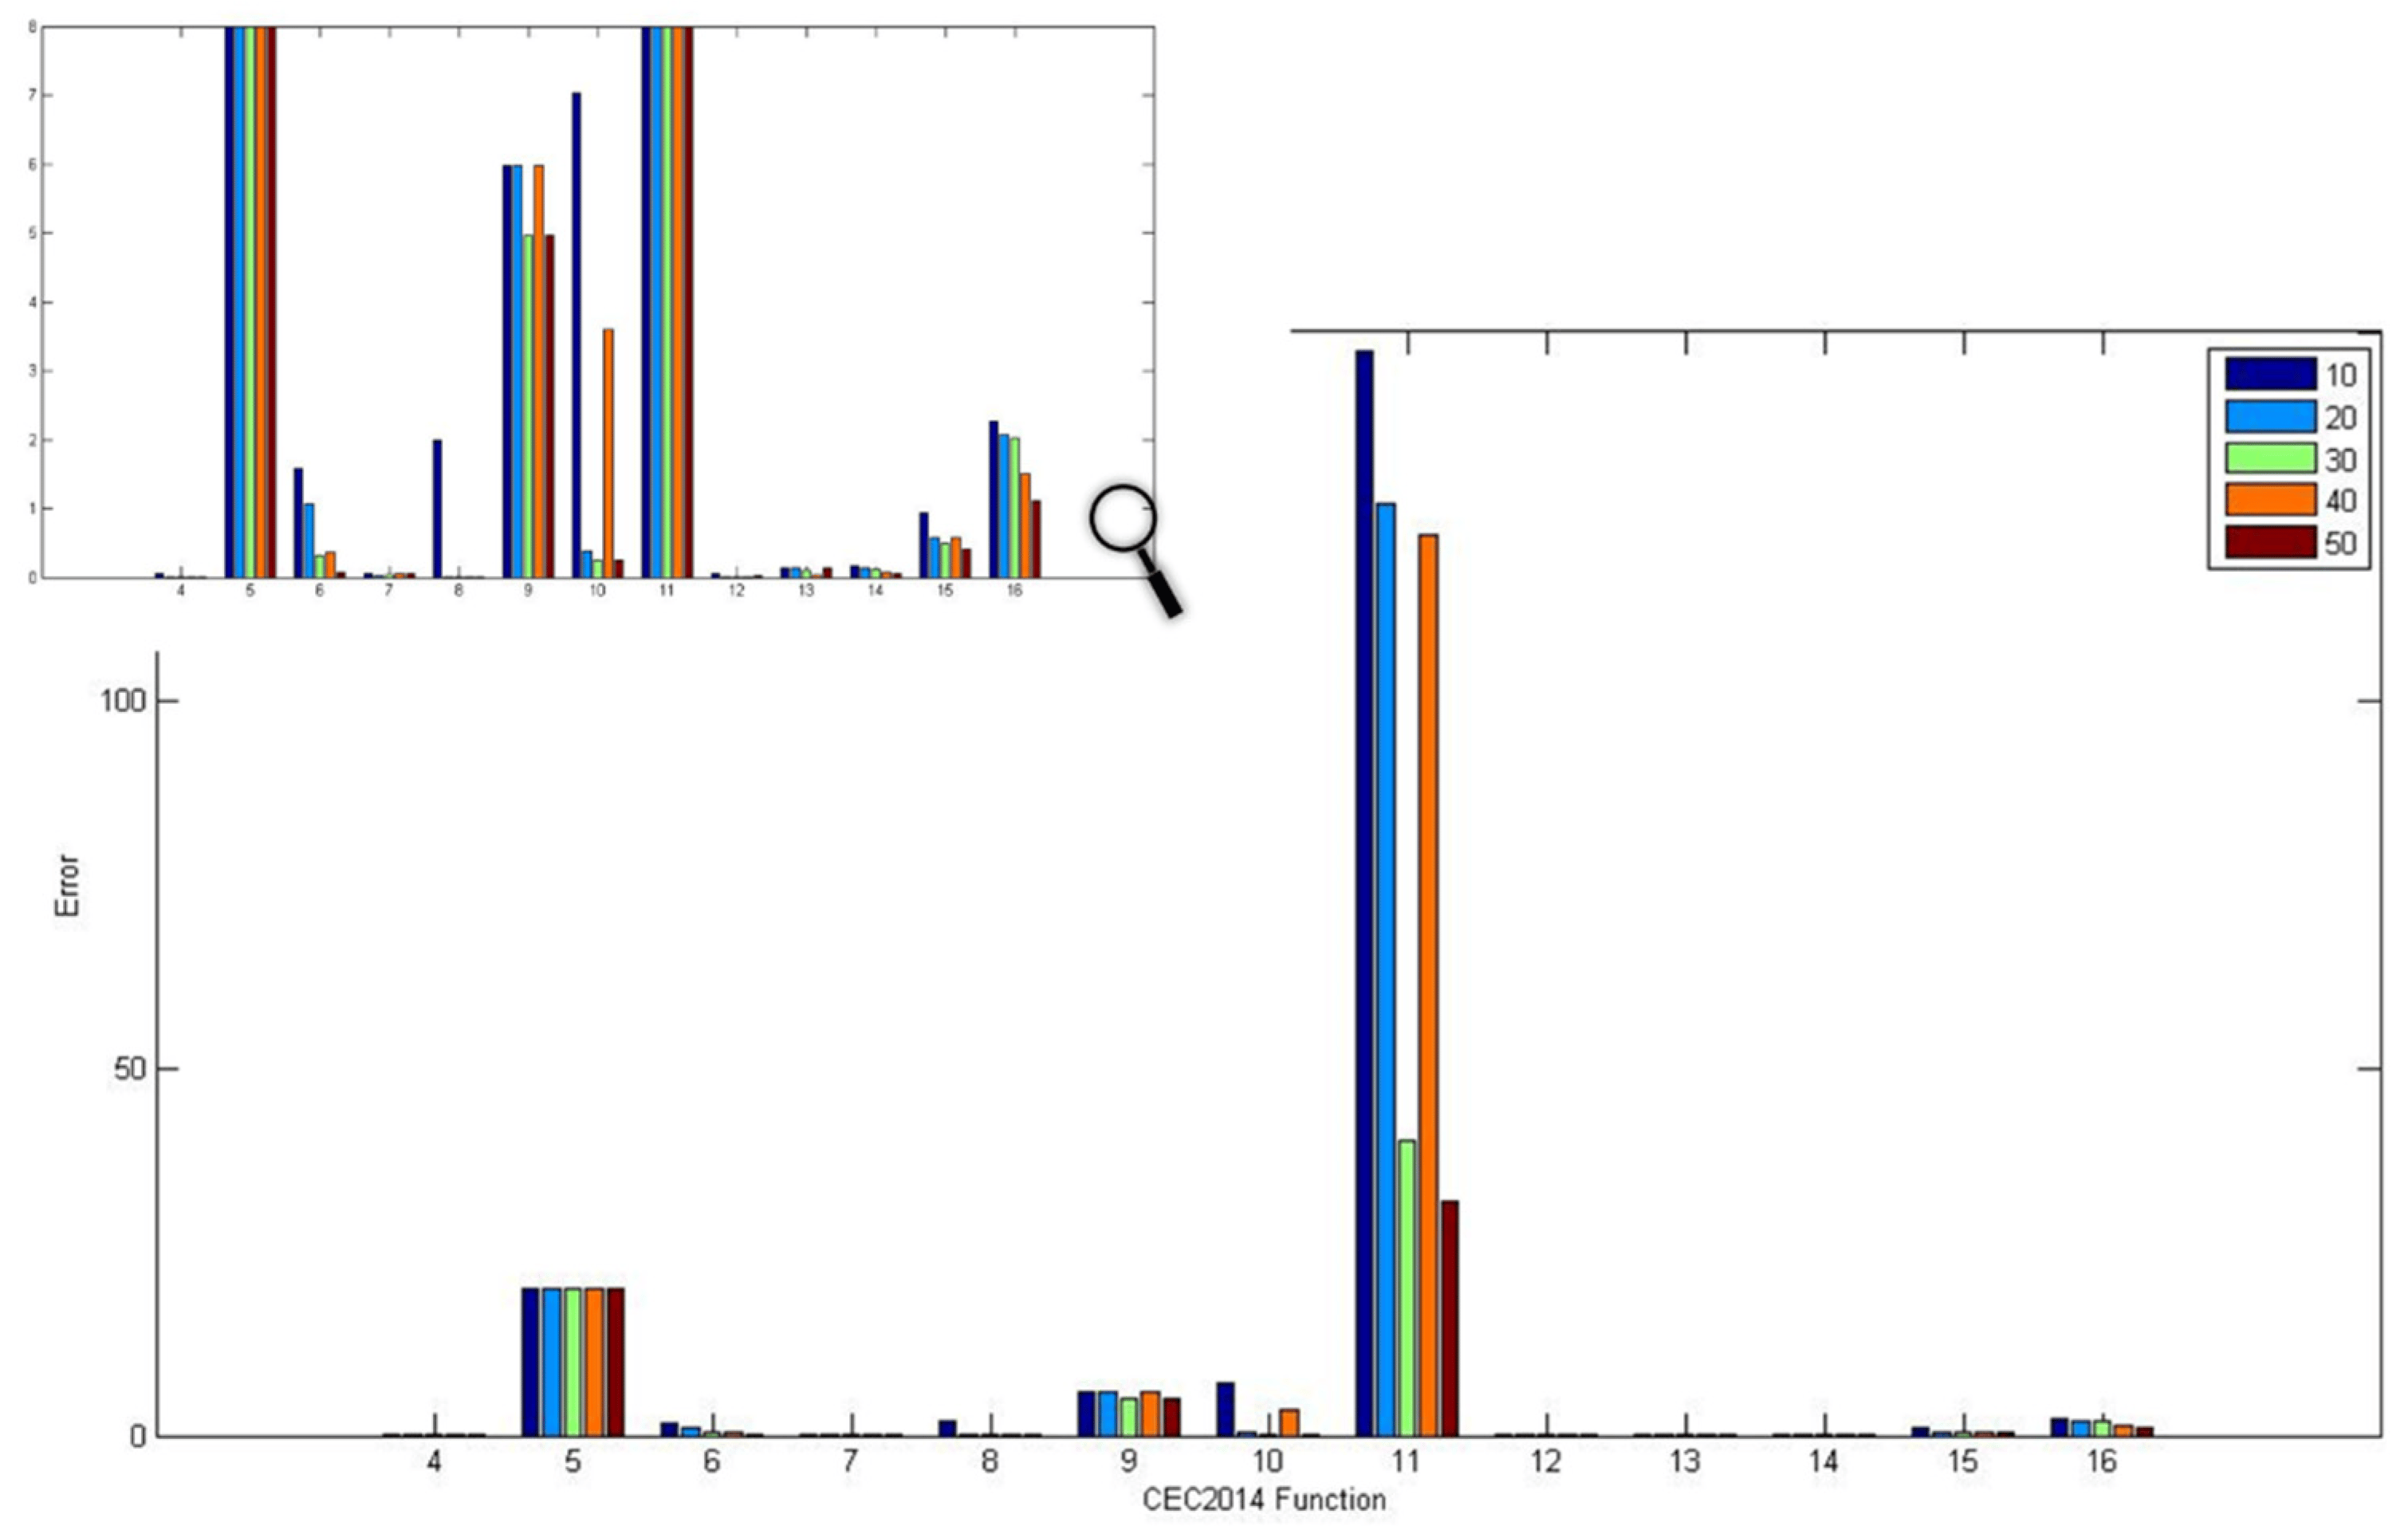
\includegraphics[width=0.5\textwidth, keepaspectratio]{Figures/image3.png}
    \caption{Error de aptitud de las funciones de referencia con diferente
        número de agentes
        \cite{aziz2022}}
    \label{fig:mi_etiqueta}
\end{figure}

Según \cite{aziz2022} la imagen 3 ilustra aún más los resultados del experimento. Los resultados se
convierten en valores de error para una mejor representación gráfica. El valor
del error es la diferencia entre la aptitud de la solución encontrada y la
aptitud ideal. En la parte superior izquierda de la figura se encuentra un
acercamiento del gráfico. Similar a lo que se observa en la Tabla 2, se puede
ver que el número de agentes igual a 50 proporciona el menor error en la
mayoría de las funciones, pero no en todas las funciones.

\section{Trabajos Relacionados}
\label{sec:TR}

El trabajo mas relacionado con este trabajo es el Algoritmo metaheuristico de
seno-coseno, el cual se utiliza para guiar la búsqueda de la solución
óptima fluctuando alrededor de la mejor solución. Para garantizar la
convergencia, dicho algoritmo envuelve la función seno y coseno usando una
función
decreciente lineal reflejada por el eje del tiempo. Sin embargo, a pesar de la
fluctuación y el sobre del decrecimiento lineal, tanto
\cite{abualigah2021advances} como \cite{gabis2021comprehensive} enumeran
la convergencia prematura como la desventaja de SCA. Además,
\cite{askari2020critical} destacó que
las ecuaciones de actualización de la solución de SCA resultan en un sesgo
hacia el origen, lo que hace que SCA funcione muy bien para problemas de
optimización donde la solución global se encuentra en el origen.
El rendimiento disminuye con los problemas desplazados. Se necesitan tres
números aleatorios en SCA.

El trabajo de \cite{aziz2022} imita un fenómeno físico, a saber, el movimiento
armónico
de un péndulo, para mover a los agentes de búsqueda de manera que se logre una
solución óptima. A diferencia de SCA, el movimiento armónico del péndulo
disminuye con la función exponencial. Se ha observado que la función
exponencial proporciona un buen equilibrio entre exploración y explotación en
metaheurísticas \cite{aziz2018singlesolution, rahman2018singleagent}. Los
agentes de algoritmo de Búsqueda del Péndulo no seleccionan aleatoriamente
entre
las funciones seno y coseno; más bien, siguen la función de movimiento
armónico. La función de movimiento armónico determina el límite máximo para los
números aleatorios que controlan la búsqueda estocástica de los agentes del
algoritmo de Búsqueda del Péndulo,
con respecto a la solución actual y la mejor solución.

\section{Conclusiones}
\label{sec:Conclusiones}
En este trabajo se presentó una propuesta de solución para optimizar la
distribución de medicamentos en centros de salud mediante la implementación de
un algoritmo de Búsqueda del Péndulo en una API Restful utilizando
Node.js y MongoDB. La solución propuesta se centró en la utilización de la
metaheurística como método de optimización y en la implementación de una
aplicación web que permita a los usuarios realizar la optimización de la
distribución de medicamentos de manera eficiente y efectiva.
Se realizó una revisión bibliográfica exhaustiva sobre los algoritmos
metaheurísticos y su aplicación en la optimización de la distribución de
medicamentos en centros de salud. Se estudió en profundidad el algoritmo de
Búsqueda del Péndulo y se propone su implementación en una API Restful
utilizando Node.js y MongoDB para la optimización de la distribución de
medicamentos.
La propuesta de solución presentada en este anteproyecto podría ser una
alternativa viable y efectiva para resolver el problema de la distribución de
medicamentos en centros de salud. La utilización de la metaheurística como
método de optimización permitiría encontrar soluciones óptimas en tiempos
razonables y con costos computacionales acotados. Además, la implementación de
una API Restful utilizando Node.js y MongoDB permitiría una fácil integración
con otras aplicaciones y sistemas existentes.
La propuesta presentada puede ser una alternativa efectiva para optimizar la
distribución de medicamentos en centros de salud. Se espera que este trabajo
sirva como una base sólida para futuros estudios y desarrollos en este campo.

\renewcommand\refname{Referencias}
\bibliographystyle{IEEEtran}
\bibliography{EjemploBIO}

\end{document}